\chapter{\MakeUppercase{Results and Discussion}}
\justifying

\section{Results Overview}

This section presents a comprehensive evaluation of the QNA-Auth system using multiple analytical perspectives, including classification performance, embedding behavior, and threshold characteristics. The objective is not only to report numerical performance but also to understand the system's behavior under realistic authentication conditions.

% -----------------------------

\section{Classification Performance}

\begin{figure}[H]
\centering
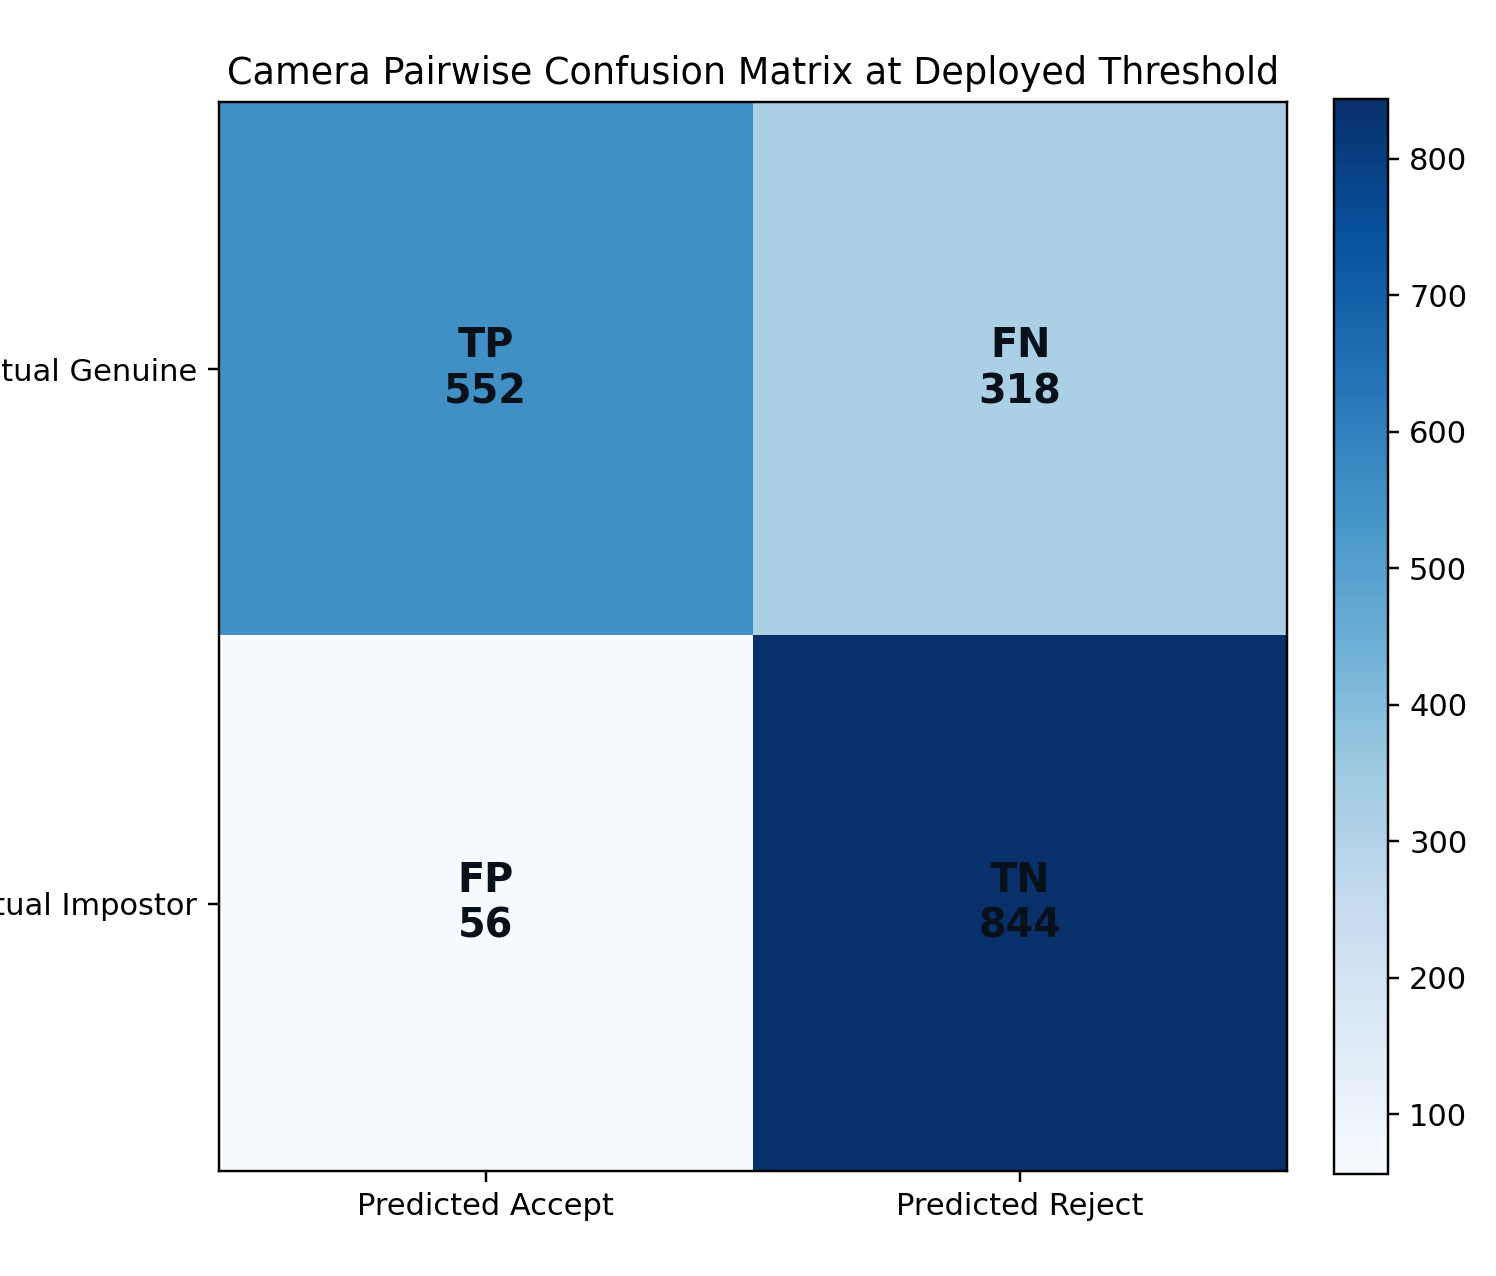
\includegraphics[width=0.75\linewidth]{images/camera_confusion_matrix.png}
\caption{Confusion matrix at deployed threshold}
\label{fig:conf_matrix}
\end{figure}

The confusion matrix demonstrates that the system is effective at distinguishing between genuine and impostor samples. A high number of true positives (552) and true negatives (844) indicates strong discrimination capability.

However, the relatively high number of false negatives (318) suggests that the system rejects a significant portion of genuine users. This behavior is a direct consequence of using a high decision threshold, which prioritizes security (low false acceptance) over usability.

% -----------------------------

\section{Embedding Space Analysis}

\begin{figure}[H]
\centering
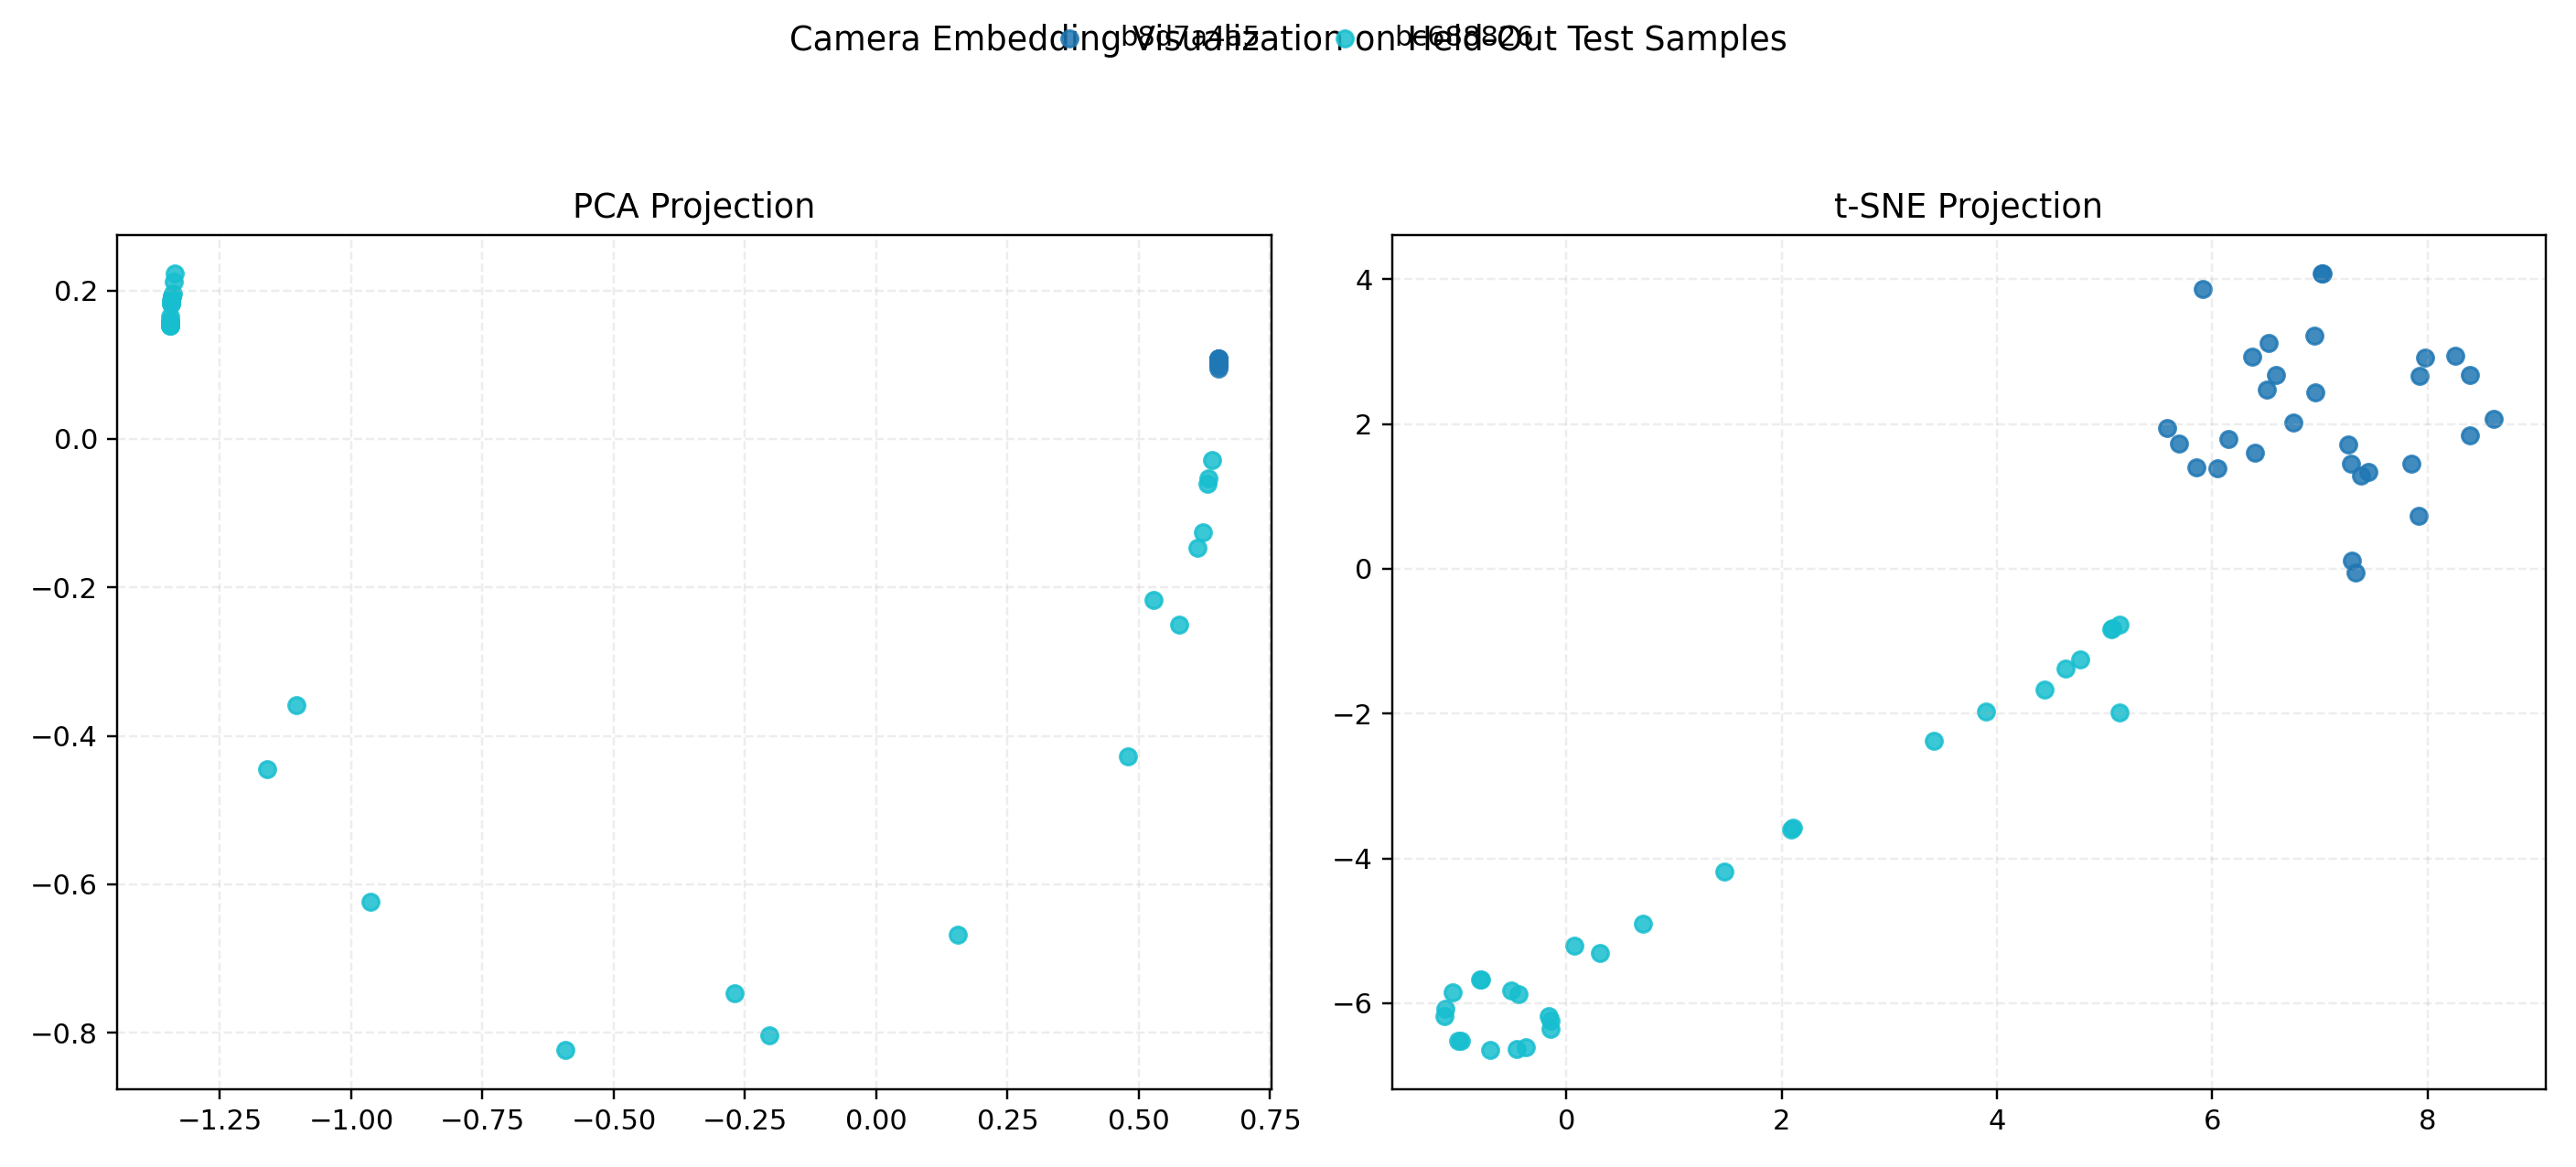
\includegraphics[width=0.95\linewidth]{images/camera_embedding_projection.png}
\caption{Embedding visualization using PCA and t-SNE}
\label{fig:embedding}
\end{figure}

The PCA and t-SNE projections show that the Siamese network learns meaningful and separable embeddings. Distinct clustering of device identities is visible, especially in the t-SNE plot, indicating that the learned feature space captures device-specific characteristics effectively.

% -----------------------------

\section{Modality Comparison}

\begin{figure}[H]
\centering
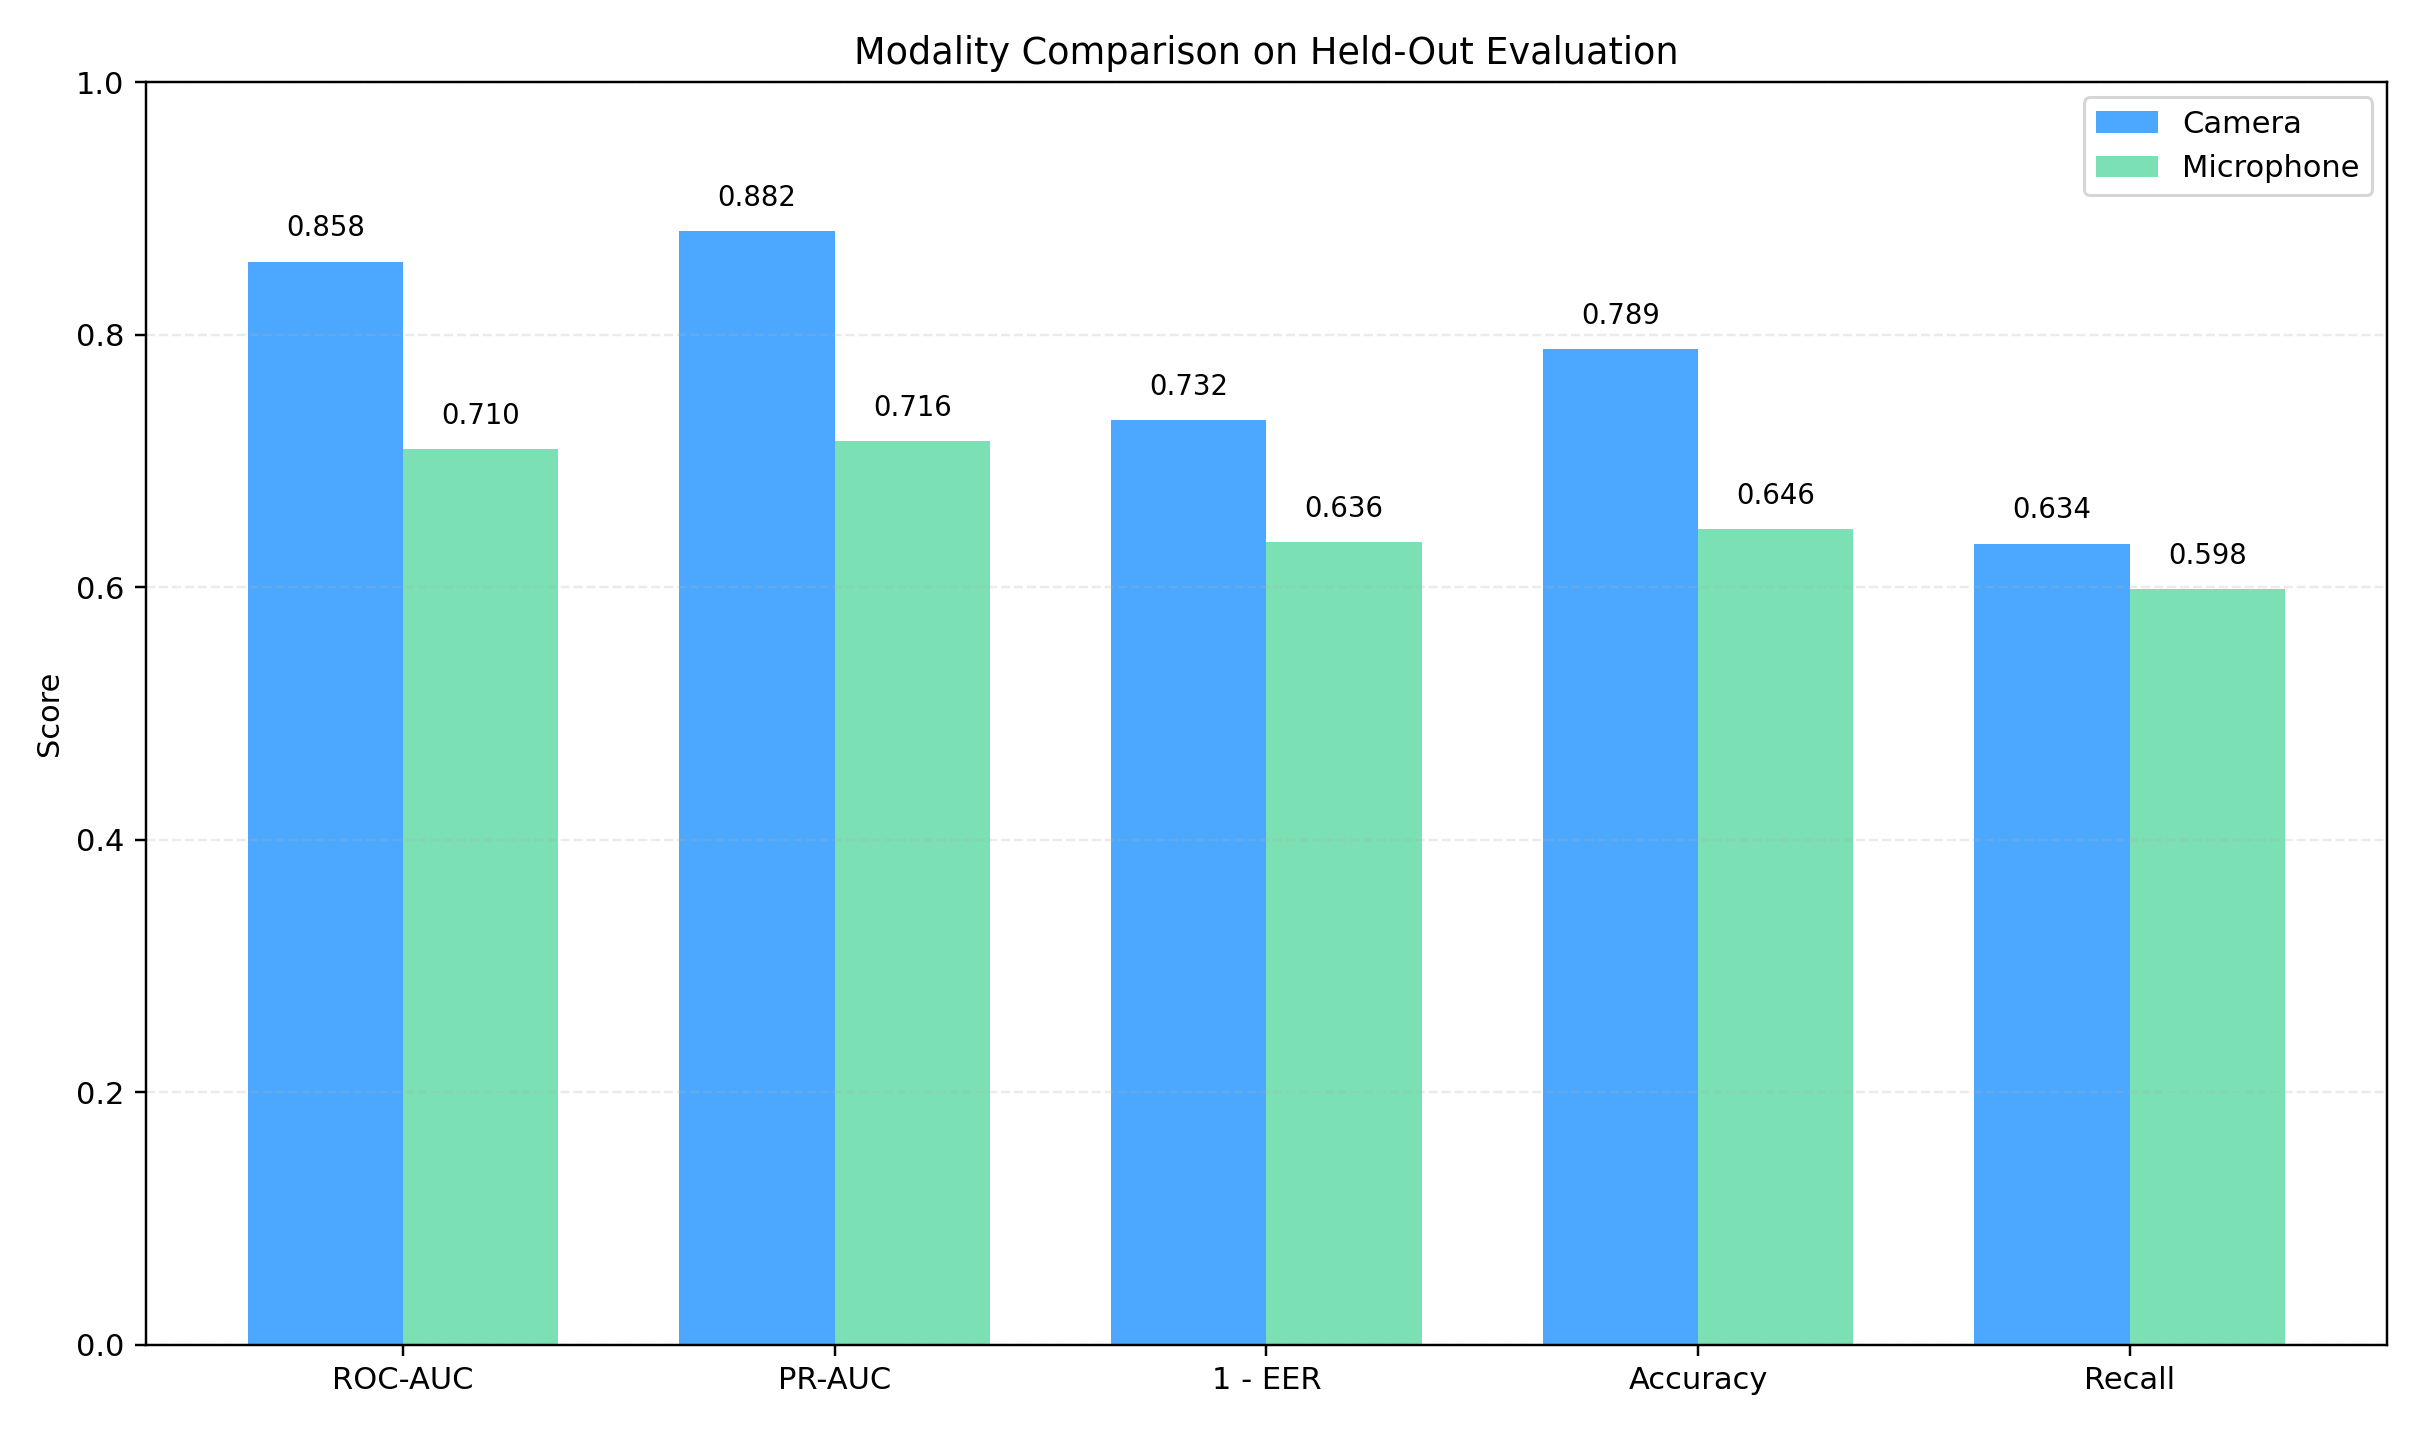
\includegraphics[width=0.85\linewidth]{images/modality_performance_comparison.png}
\caption{Performance comparison between camera and microphone modalities}
\label{fig:modality}
\end{figure}

The comparison shows that camera-based features outperform microphone-based features across all evaluation metrics. This suggests that camera sensor noise provides more stable and discriminative patterns for device identification.

% -----------------------------

\section{Comparison with Prior Work}

\begin{table}[H]
\centering
\caption{Comparison of QNA-Auth with prior device fingerprinting approaches}
\label{tab:comparison}
\renewcommand{\arraystretch}{1.3}
\begin{tabular}{|p{4cm}|p{2cm}|p{2cm}|p{2cm}|p{2cm}|p{2cm}|}
\hline
\textbf{Method} & \textbf{Modality} & \textbf{ROC-AUC} & \textbf{EER} & \textbf{Accuracy} & \textbf{Replay Protection} \\
\hline

Lukas et al. (2006) — PRNU & Camera & $\sim$0.95+ & $\sim$4\% & $\sim$96\% & None \\
\hline

Goljan et al. (2009) — Large-scale PRNU & Camera & $\sim$0.97+ & $\sim$2.5\% & $\sim$97\% & None \\
\hline

Chen et al. (2008) — ML-PRNU & Camera & $\sim$0.96+ & $\sim$2\% & $\sim$97\% & None \\
\hline

Das et al. (2014) — Acoustic fingerprint & Microphone & $\sim$0.82 & $\sim$9\% & $\sim$85\% & None \\
\hline

\textbf{QNA-Auth (Camera)} & Camera & \textbf{0.858} & \textbf{26.8\%} & \textbf{78.9\%} & HKDF nonce \\
\hline

\textbf{QNA-Auth (Microphone)} & Microphone & \textbf{0.710} & \textbf{36.4\%} & \textbf{64.6\%} & HKDF nonce \\
\hline

\end{tabular}
\end{table}

The comparison shows that classical PRNU-based approaches achieve higher accuracy under controlled conditions. However, these methods operate in offline forensic settings and do not incorporate real-time authentication constraints.

In contrast, QNA-Auth is designed as a deployable system, incorporating real-time capture, noisy environments, and security mechanisms such as nonce-based replay protection.

% -----------------------------

\section{Measured and Projected Future Results}

The repository now contains two distinct result categories that should be kept separate in the thesis narrative. First, there are measured results already saved under \texttt{model/evaluation/} and \texttt{artifacts/capstone\_eval/}. Second, there is a forecast bundle under \texttt{Predicted report/} that estimates what a larger, multi-session fused system could achieve in future work.

\begin{table}[H]
\centering
\caption{Measured and projected QNA-Auth result summary}
\label{tab:measured_projected_summary}
\renewcommand{\arraystretch}{1.3}
\begin{tabular}{|p{4.2cm}|p{1.7cm}|p{1.7cm}|p{1.7cm}|p{1.7cm}|}
\hline
\textbf{Configuration} & \textbf{ROC-AUC} & \textbf{EER} & \textbf{Accuracy} & \textbf{Claim Type} \\
\hline
QNA-Auth (Camera measured) & 0.858 & 26.8\% & 78.9\% & Measured \\
\hline
QNA-Auth (Microphone measured) & 0.710 & 36.4\% & 64.6\% & Measured \\
\hline
QNA-Auth (April 22 capstone artifact) & N/A & 10.0\% & 83.3\% & Measured \\
\hline
QNA-Auth (Fused conservative scenario) & 0.900 & 12.0\% & 85.0\% & Projected \\
\hline
QNA-Auth (Fused target scenario) & 0.930 & 8.0\% & 89.0\% & Projected \\
\hline
QNA-Auth (Fused stretch scenario) & 0.950 & 6.0\% & 92.0\% & Projected \\
\hline
\end{tabular}
\end{table}

The projected rows are not claimed as measured output. They are scenario estimates derived from the current artifact range and from the expected benefit of larger device diversity, repeated sessions, validation-calibrated thresholds, and camera-dominant fusion. This distinction matters because the thesis must show both current evidence and the future viability path without conflating the two.

\begin{figure}[H]
\centering

\includegraphics[width=0.82\linewidth]{\detokenize{../../Predicted report/images/measured_vs_projected_metrics.png}}
\caption{Measured modality performance versus projected fused target performance}
\label{fig:measured_projected_bar}
\end{figure}

\begin{figure}[H]
\centering

\includegraphics[width=0.76\linewidth]{\detokenize{../../Predicted report/images/projected_roc_curves.png}}
\caption{Projected ROC curves for future fusion scenarios}
\label{fig:projected_roc_ch7}
\end{figure}

% -----------------------------

\section{Overall Discussion}

The results demonstrate that QNA-Auth successfully captures device-specific characteristics using sensor noise and can distinguish between genuine and impostor samples with reasonable effectiveness.

The system exhibits strong impostor rejection (low FAR), but higher false rejection rates indicate sensitivity to threshold selection and environmental variability. This highlights the inherent trade-off between security and usability.

Additionally, the system's performance varies across modalities, with camera-based fingerprinting proving more reliable than microphone-based approaches.

The projected future results strengthen the viability argument without changing the evidentiary boundary. They show that, if the dataset is expanded and calibrated fusion is evaluated under stronger split discipline, the system could move from a promising prototype toward a more competitive short-sample verification pipeline. That is an academically useful conclusion because it explains why the project is worth continuing, even though the current measured results remain bounded.

\section{Conclusion of Results}

Overall, the proposed system validates the feasibility of sensor-based device authentication in a practical setting. While not yet matching the performance of controlled forensic methods, it demonstrates a meaningful step toward real-world deployment by integrating machine learning, signal processing, and security-aware system design.
